\chapter{Material y método}
\section{Diseño de la investigación}
Estudio de enfoque cuantitativo, diseño analítico, prospectivo de corte
transversal.

\section{Población}
	\begin{enumerate}
		\item Población o universo: Niños menores de 5 años en el área de salud
		del distrito de Quetzaltenango.
		\item Marco muestral: Niños menores de 5 años que acuden a servicios de
		atención primaria en el Puesto de Salud de San José Chiquilajá, Puesto
		de Salud de Pacajá y el Centro de Salud de Quetzaltenango. 
		\item Muestra: \muestradeseada\ niños menores de 5 años que acudan a
		servicios de atención primaria seleccionados en Quetzaltenango.
	\end{enumerate}

\section{Tamaño de muestra}
El tipo de muestreo fue no probabilístico por conveniencia, se incluyeron a
todos los niños que cumplieron con los criterios de inclusión y asistieron a
servicios de atención primaria, hasta alcanzar el tamaño de muestra deseado
de \muestradeseada\ niños.

\section{Unidad de análisis}
	\begin{enumerate}
		\item Unidad primaria de muestreo: Servicios de atención primaria en
		salud de la ciudad de Quetzaltenango, en específico el Puesto de
		Salud de San José Chiquilajá, Puesto de Salud de Pacajá y el Centro de
		Salud de Quetzaltenango.
		\item Unidad de análisis: Información sobre aspectos sociodemográficos,
		económicos, familiares, perinatales, nutricionales, médicos, de
		interacción y estimulación de los niños y su evaluación de riesgo de
		acuerdo a los dominios del desarrollo de comunicación, área motora
		gruesa y fina, resolución de problemas y área socio-individual.
		\item Unidad de información: Madres o encargados y niños que acudan a
		servicios de atención primaria de la ciudad de Quetzaltenango.
	\end{enumerate}

\section{Hipótesis}
	\begin{enumerate}
		\item Hipótesis nula (H0): No existe una asociación significativa entre
		factores sociodemográficos, condiciones económicas, interacción
		familiar, exposición a dispositivos electrónicos, antecedentes médicos
		perinatales y postnatales, y el riesgo en el neurodesarrollo de niños
		menores de 5 años en servicios de atención primaria de Quetzaltenango.
		\item Hipótesis alternativa (H1): Existe una asociación significativa
		entre factores sociodemográficos, condiciones económicas, interacción
		familiar, exposición a dispositivos electrónicos, antecedentes médicos
		perinatales y postnatales, y el riesgo en el neurodesarrollo de niños
		menores de 5 años en servicios de atención primaria de Quetzaltenango.
	\end{enumerate}

\section{Criterios de inclusión y exclusión}
	\begin{enumerate}
		\item Criterios de inclusión:
			\begin{itemize}
				\item Niños de 0 a 59 meses de edad que acuden a servicios de
				atención primaria para controles de crecimiento y desarrollo,
				vacunación o consulta médica.
				\item Padres o cuidadores que acepten participar en el estudio
				y firmen el consentimiento informado.
			\end{itemize}
		\item Criterios de exclusión:
			\begin{itemize}
				\item Niños con diagnóstico previo de trastornos del
				neurodesarrollo o discapacidad intelectual
				\item Padres o cuidadores que no acepten participar en el
				estudio o se retiren durante el proceso.
			\end{itemize}
	\end{enumerate}

\section{Definición y operacionalización de variables}
Las variables cualitativas incluyen: sexo, etnia, residencia, escolaridad del
cuidador, servicios básicos como agua, servicios sanitarios, eliminación de
basura y alumbrado, propiedad de casa, condición y tipo de empleo, estado civil,
tipo de parto y atención del mismo.

Las variables cuantitativas comprenden: edad (intervalos: años, meses), número
de personas en casa y hermanos (discretas), exposición a dispositivos
electrónicos y tiempo de juego cuidador-niño (continuas) controles prenatales
(discreta), y los cinco dominios del neurodesarrollo evaluadas mediante
cuestionarios (cuantitativas de escala).

Se describen de forma ordenada en la siguiente tabla:

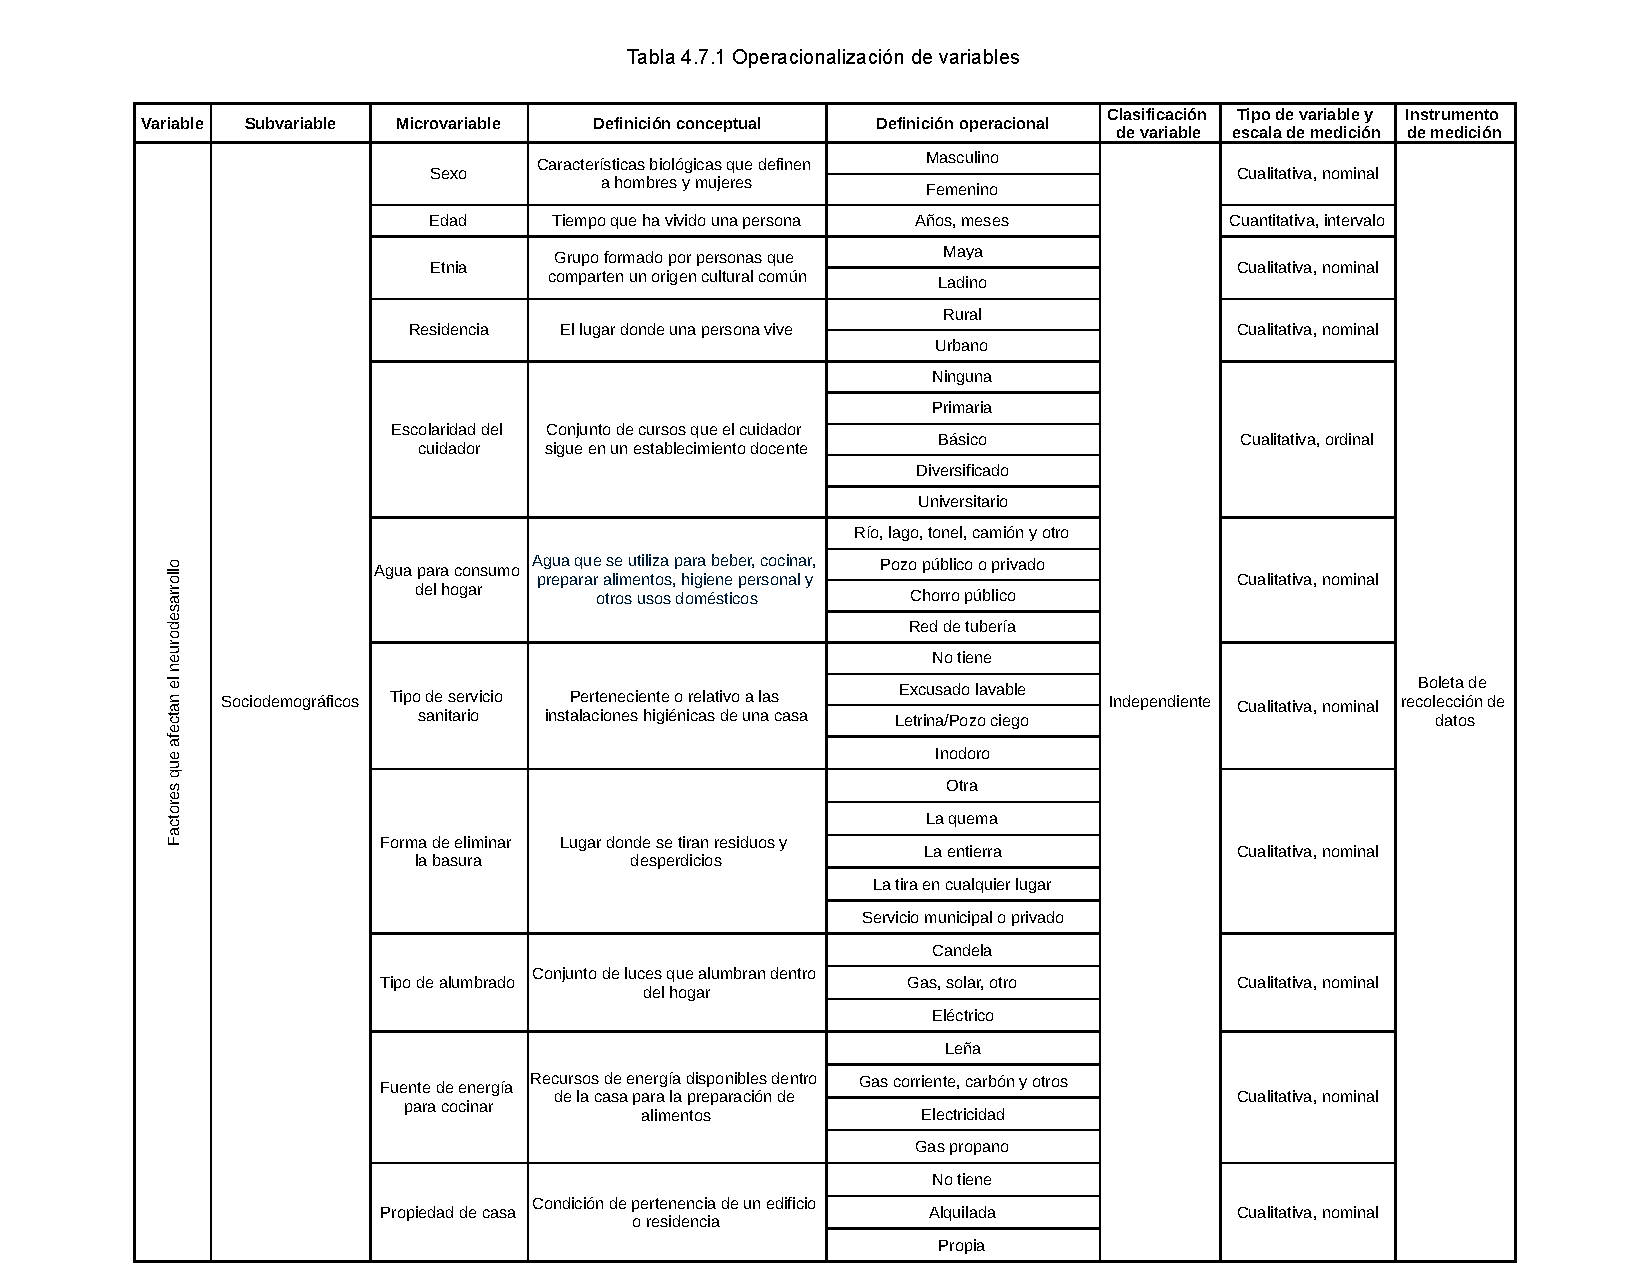
\includepdf[scale=0.93,landscape=true,pages=-,pagecommand={\thispagestyle{plain}}]{images/variables.pdf}

\section{Instrumentos utilizados en la recolección de la información}
Para este estudio se emplearon los siguientes instrumentos:
		\begin{itemize}
		\item \asq: Adaptado al idioma español y ajustado por edad.	
		\item Cuestionario de factores de riesgo.
		\end{itemize}

\section{Procedimientos para la recolección de información}
	\begin{enumerate}
		\item Fase preliminar:
		Se obtuvieron los permisos correspondientes a las autoridades de salud
		del departamento de Quetzaltenango para acceder a los servicios de
		atención primaria seleccionados. Se determinaron estrategias para
		garantizar la uniformidad en la recolección de los datos entre los
		investigadores.
		\item Fase de recolección de datos:
		Se identificaron niños menores de 5 años que cumplieron con los
		criterios de inclusión en los servicios de atención primaria
		participantes. Tras obtener el consentimiento informado de los padres o
		tutores, se realizó:
			\begin{itemize}
			\item Evaluación del neurodesarrollo mediante la aplicación del
			\asq, seleccionando la versión específica según la edad del niño.
			\item Aplicación de un cuestionario estructurado para recolectar
			información sobre factores potencialmente asociados al
			neurodesarrollo.
			\end{itemize}
		\item Fase de clasificación y análisis:
		Los resultados de cada niño fueron evaluados conforme al puntaje
		obtenido en el \asq\ y clasificados en tres categorías:
			\begin{itemize}
			\item Desarrollo típico: puntaje en el área blanca, indicativo de
			un desarrollo acorde a su edad.
			\item Requiere monitoreo: puntaje en el área gris, señalando
			habilidades ligeramente por debajo del promedio.
			\item Retraso en el desarrollo: puntaje en el área negra,
			sugiriendo la necesidad de intervención especializada.
			\end{itemize}
		Se analizaron las asociaciones entre los factores de exposición
		identificados y los resultados de neurodesarrollo en la evaluación.
	\end{enumerate}

\section{Procedimientos de análisis de la información}
Los datos fueron recolectados utilizando la boleta de recolección de datos (ver
anexo D) la cual consiste en un formulario en línea.

Se realizó una limpieza inicial de datos para asegurar la consistencia de los
datos y evitar sesgo por entrada de datos.

Los puntajes obtenidos en cada área del desarrollo del \asq\ se convirtieron a
puntajes Z de acuerdo con la ficha técnica de los cuestionarios. 
	
\subsection{Análisis descriptivo}
Se realizó un análisis descriptivo de la muestra, calculando frecuencias y
porcentajes para las variables categóricas, y medidas de tendencia central y
dispersión para las variables cuantitativas.

\subsection{Análisis inferencial}
Para evaluar la asociación entre los factores de riesgo (variables
independientes) y los resultados del \asq\ (variables dependientes), se
aplicaron las siguientes técnicas estadísticas:

\subsubsection{Prueba Chi-cuadrado de independencia}
Se utilizó esta prueba para analizar la asociación entre factores de riesgo
categóricos y los resultados del \asq\ dicotomizados (desarrollo adecuado/en
riesgo) y determinar la significancia estadística.

Para una población de \muestradeseada\ niños menores de 5 años, el
procedimiento para la prueba Chi-cuadrado fue el siguiente:

\begin{itemize}
    \item Se realizaron tablas de contingencia para cada par de variables
		categóricas (factor de riesgo y resultado del \asq).
    
    \item Se calculó el estadístico Chi-cuadrado mediante la fórmula:
    \[
    \chi^2 = \sum_{i=1}^r \sum_{j=1}^c \frac{(O_{ij} - E_{ij})^2}{E_{ij}}
    \]
    
    Donde \( O_{ij} \) son las frecuencias observadas y \( E_{ij} \) son las
	frecuencias esperadas bajo la hipótesis nula de independencia.
    
    \item Se estableció un nivel de significancia estadística de $\alpha = 0.05$
		para todas las pruebas, e intervalos de confianza de 95\% cálculados
		por el método del error estándar para describir el rango en el que se
		encuentra el valor real.
\end{itemize}

\subsection{Análisis de varianza (ANOVA)}
Para evaluar la relación entre factores de riesgo con múltiples categorías y
los resultados del neurodesarrollo cuantificados mediante puntajes Z del 
\asq, se utilizó el análisis de varianza (ANOVA) de una vía. Se utilizó esta
técnica estadística para determinar si existen diferencias significativas en las
medias de los puntajes Z entre tres o más grupos independientes, definidos por
las distintas categorías de los factores de riesgo.

El modelo matemático del ANOVA de un factor puede expresarse como:

\begin{equation}
Y_{ij} = \mu + \alpha_i + \varepsilon_{ij}
\end{equation}

Donde:
\begin{itemize}
    \item $Y_{ij}$ es la observación $j$-ésima en el $i$-ésimo grupo
    \item $\mu$ es la media general
    \item $\alpha_i$ es el efecto del factor de riesgo $i$
    \item $\varepsilon_{ij}$ es el error aleatorio que sigue una distribución $N(0, \sigma^2)$
\end{itemize}

El estadístico $F$ para el ANOVA se calcula como la razón entre la varianza
entre grupos y la varianza dentro de los grupos:

\begin{equation}
F = \frac{MS_{\text{entre}}}{MS_{\text{dentro}}} = \frac{\sum_{i=1}^{k} n_i(\bar{Y}_i - \bar{Y})^2/(k-1)}{\sum_{i=1}^{k}\sum_{j=1}^{n_i} (Y_{ij} - \bar{Y}_i)^2/(N-k)}
\end{equation}

Donde:
\begin{itemize}
    \item $MS_{\text{entre}}$ es la media cuadrática entre grupos
    \item $MS_{\text{dentro}}$ es la media cuadrática dentro de los grupos
    \item $k$ es el número de grupos
    \item $n_i$ es el tamaño de la muestra del grupo $i$
    \item $\bar{Y}_i$ es la media del grupo $i$
    \item $\bar{Y}$ es la media general
    \item $N$ es el tamaño total de la muestra
\end{itemize}

Dado que los tamaños muestrales no son homogéneos entre los diferentes grupos de
interés (debido a las características propias del muestreo en servicios de
atención primaria), se aplicó la prueba de Levene para evaluar si la
heterogeneidad de los resultados era significativa. 

\subsubsection{Prueba de Levene para homogeneidad de varianzas}
La prueba de Levene es una prueba estadística inferencial utilizada para
evaluar la igualdad de varianzas entre diferentes grupos. Esta prueba es menos
sensible a desviaciones de la normalidad que otras pruebas de igualdad de
varianzas, lo que la hace particularmente útil en el contexto de este estudio.

El procedimiento de la prueba de Levene implica:
\begin{itemize}
    \item Calcular la diferencia absoluta entre cada valor en un grupo y la
		media o mediana de ese grupo.
    \item Realizar un ANOVA de un factor sobre estos valores de diferencia
		absoluta.
    \item El estadístico resultante sigue una distribución F con k-1 y N-k
		grados de libertad, donde k es el número de grupos y N el tamaño total
		de la muestra.
\end{itemize}

Se interpretó el valor p de la prueba de Levene de la siguiente manera:
\begin{itemize}
    \item Si $p > 0.05$: No se rechaza la hipótesis nula de igualdad de
		varianzas, por lo que se procede con el ANOVA tradicional.
    \item Si $p \leq0.05$: Se rechaza la hipótesis nula, lo que indica que las
		varianzas no son iguales entre los grupos.
\end{itemize}

En caso de que no se cumpliera el supuesto de homogeneidad de varianzas, se
utilizó la prueba de Welch como alternativa al ANOVA tradicional. La prueba de
Welch realiza un ajuste de los grados de libertad para compensar la
heterogeneidad de varianzas, lo que la hace especialmente apropiada para
muestras con tamaños desiguales.

\subsubsection{Análisis post-hoc}
En los casos donde se encontraron diferencias significativas en el ANOVA
($p < 0.05$), se realizaron pruebas post-hoc Tukey HSD para identificar
específicamente entre qué grupos existen las diferencias.

\subsection{Análisis de asociación}
Se analizaron los resultados del \asq\ del grupo estudiado utilizando odds
ratio (OR): para comparar las probabilidades de que se presente riesgo en el
neurodesarrollo entre dos grupos diferentes. Por ejemplo, para comparar si los
niños con padres que tienen un trabajo formal o informal tienen mayor
probabilidad o no, de presentar riesgo en el neurodesarrollo.

\subsection{Presentación de resultados}
Se elaboraron tablas y gráficos apropiados con intervalos utilizando python y
paquetes numpy, pandas, también se utilizó el software rstudio con paquetes de
CRAN.

\section{Procedimientos para garantizar aspectos éticos de la investigación}
El presente estudio cumplió con los principios éticos fundamentales establecidos
para la investigación en seres humanos, se garantizó la protección de los
derechos, dignidad y bienestar de los participantes. A continuación, se
detallan los aspectos éticos considerados:

\subsection{Respeto por las personas}
Se aseguró el respeto a la autonomía de los cuidadores y los participantes al
obtener su consentimiento informado previo a la participación en el estudio.
En este documento se describieron claramente los objetivos, procedimientos,
beneficios y posibles riesgos del estudio.

\subsection{Confidencialidad y privacidad}
La privacidad de los participantes se respetó de forma estricta. Toda la
información recolectada fue tratada de manera confidencial y utilizada
únicamente con fines de investigación.

\subsection{Justicia}
Se garantizó que todos los niños elegibles tuviesen igualdad de oportunidades
para participar en el estudio, sin discriminación por razones de género, etnia,
nivel socioeconómico o creencias religiosas. Asimismo, los resultados del
estudio están orientados a beneficiar a la comunidad en general, fomentando
políticas y estrategias que mejoren el neurodesarrollo infantil.

\subsection{Beneficencia y no maleficencia}
Este estudio no implicó intervenciones invasivas ni riesgos significativos para
los participantes. Se emplearon técnicas observacionales y cuestionarios
validados que no afectan la salud o el bienestar de los niños ni de sus
cuidadores.

\subsection{Categoría de riesgo}
Categoría I: El diseño del estudio se basó en la aplicación del \asq\ el cual
es una herramienta validada y no invasiva para evaluar el neurodesarrollo
infantil. Este cuestionario se aplicó a los cuidadores (padres o tutores) de
los niños de forma observacional y no requirió intervención directa sobre los
participantes.

\subsection{Consentimiento informado}
Todos los cuidadores firmaron un consentimiento informado (ver anexo C) antes de
participar en el estudio.
